\documentclass[10pt,a4paper]{article}
\usepackage[utf8]{inputenc}
\usepackage{amsmath}
\usepackage{amsfonts}
\usepackage{amssymb}
\usepackage{bm}
\usepackage{hyperref}
\usepackage{graphicx}
\usepackage{notestyle}
\author{A. Jakovac}
\title{NeuronLearning documentation}
\date{\today}
\begin{document}

\section{General structure}

The goal of the NeuronLearning project is to demonstrate that a a neural network can be taught without comparison to a final result.

The basic structure is expressed in the Network class. It has a hierarchical build:
\begin{itemize}
\item axons: this is the most basic block
\item layer: this provides the geometry for axons.
\item connection: establishes connections between layers
\item update: provides an update function for each layer
\end{itemize}

Once we have a network that works effectively enough, we may add some other "skins" to it that specifies the way we can use it.

\section{Backpropagation}

When we want to do supervised learning, then the result of the last layer should be compared to an expected output. The result of the comparison is quantified by some loss function $y$. The goal of the learning is to minimize the loss over the training set. For that we have to know, in which direction should we change the parameters of the network in order to improve the loss. For that we have to know the derivative of the loss with respect to the parameters. 

The loss $L$ is formally a function of the input layer ($x_0$) and the parameters of the network ($w$), i.e. $L(w, x_0)$. We would need
\begin{equation}
\frac{\partial L}{\partial w_a}.
\end{equation}

In general the derivatives can be computed one-by-one. But in a neural network we have a hierarchical structure. Let us denote the value of the $i$th axon by $x_i$. If $x$ is changed, then also $y$ changes, and we may want to compute
\begin{equation}
z_i = \frac{\partial L}{\partial x_i},
\end{equation}
Once we know these values, then the quantity of interest can be computed as (here and later on we suppress the notation of any sums) 
\begin{equation}
\frac{\partial L}{\partial w_a} = \frac{\partial L}{\partial x_i} \frac{\partial x_i}{\partial w_a} = z_i \frac{\partial x_i}{\partial w_a}.
\end{equation}
Usually a parameter is local, so there is only a single $z_i$ that contributes in the above expression.

In a hierarchical structure $y$ does not depend \emph{directly} on $x_i$, only through some other $x_j$ which are higher in the hierarchy. If we want to quantify this statement, we compose the index $i$ from two parts $i=(n,a)$ where $n$ is the layer level and $a$ is the position within the layer. An axon $x_j$ is at higher hierarchy than $x_i$ if its layer level is larger, i.e. $j_1>i_1$. But this composition may remain hidden in the notation. We simply write
\begin{equation}
\label{eq:f1}
\frac{\partial y(x_i)}{\partial x_i} = \frac{\partial y(x_j(x_i))}{\partial x_i} =\frac{\partial y}{\partial x_j} \frac{\partial x_j}{\partial x_i},
\end{equation}
which means
\begin{equation}
\label{eq:f2}
z_i = z_j \frac{\partial x_j}{\partial x_i},\qquad \mathrm{where}\; j_1>i_1.
\end{equation}
The derivative ${\partial x_j}/{\partial x_i}$ can be explicitly computed by knowing the connection between the axons. Then the above equation tells up that we can compute $z_i$, if we know all derivatives $z_j$ at \emph{higher} levels. This is the method of \emph{backpropagation}.

\subsection{Affine plus nonlinear layers}

For example if the rule of getting from one layer to another is
\begin{equation}
x_j= f_j\left(M_{ji} x_i + b_j \right),
\end{equation}
then
\begin{equation}
\frac{\partial y}{\partial x_i} = \frac{\partial y}{\partial x_j} \frac{\partial x_j}{\partial x_i} = \frac{\partial y}{\partial x_j} f_j(M_{ji} x_i + b_j) M_{ji}.
\end{equation}
So we find
\begin{equation}
z_i = z_j f'_j(M_{ji} x_i + b_j) M_{ji}.
\end{equation}
Moreover
\begin{eqnarray}
&& \frac{\partial y}{\partial M_{ji}} = \frac{\partial y}{\partial x_j} \frac{\partial x_j}{\partial M_{ji}} = z_j f'_j(M_{ji} x_i + b_j) x_i \nn
&& \frac{\partial y}{\partial b_j} = \frac{\partial y}{\partial x_j} \frac{\partial x_j}{\partial b_j} = z_j f'_j(M_{ji} x_i + b_j).
\end{eqnarray}

Technically it is possible to compute $f'_j(M_{ji} x_i + b_j)$ at the same time when $x_j=f_j(M_{ji} x_i + b_j)$ is computed. But if we want apply backpropagation as a skin, we should have a function that determines $f'$ from the value of $x_j$, which is already stored in the axon variable. It is possible if $f$ is invertible:
\begin{equation}
f'_j(M_{ji} x_i + b_j) = f'_j( f_j^{-1}(x_j) ) \stackrel != df_j(x_j).
\end{equation}
To have some examples:
\begin{eqnarray}
&& f(x) = \Theta(x) x \tehat df = \Theta(f>0)\qquad \mbox{ (\texttt{ReLU}) }\nn
&& f(x) = \alpha \tanh(\beta x) \tehat f'(x) = \alpha\beta \left( 1- \frac{f^2}{\alpha^2} \right),\nn
&& f(x) = \alpha \exp(\beta x) \tehat f'(x) = \beta x,\nn
&& f(x) = x|_{\mathrm{largest}}\tehat f'(x)=1|_{\mathrm{largest}}\qquad \mbox{ (\texttt{maxpool}) }.
\end{eqnarray}
In case of maxpool there is no parameters for the connection strength. In order to be treated in a uniform way, however, we require that the update funtion should set all of the $M_{ji}=0$, except for the largest $x$, where it is $1$. It is then ensured that the derivative propagates back only for the largest value.

In this way we have the recursions for $j_1>i_1$:
\begin{eqnarray}
&& \frac{\partial y}{\partial b_j} = z_j df_j(x_j),\quad
   \frac{\partial y}{\partial M_{ji}} = z_j df_j(x_j) x_i\nn
&& z_i = z_i+ z_j df_j(x_j) M_{ji},\quad \mathrm{starting\ from\ } z_i =0.
\end{eqnarray}
Then we can maintain the effectivity of the code as well as the modularity. 

\subsection{Loss functions and derivatives}

The last layer is special, since it is directly connected to the loss function. In this case there are no parameters, backpropagation only propagates the derivative to its input sites. The loss is always a result of the comparison of the actual output $x$ and the expected output $\bar x$.

Sometimes the loss is used on normalized output. This means that we compute $L(x)=\ell(\dfrac{x}{X})$, where $X=\sum_i x_i$. Its derivative reads
\begin{equation}
\dfrac{\partial L}{\partial x_i} =  \frac1X \left ( \partial_i\ell - C \right ),\qquad \mathrm{where} \quad C=\dfrac{1}{X} \sum_j x_j\partial_j \ell,
\end{equation}
$C$ is a constant. The last term ensures that $\sum_i x_i \partial_i L =0$.

The most simple function is the p-norm loss function
\begin{equation}
\ell_p(x) = \dfrac{1}{p} \sum_i |x_i -\bar{x_i}|^p,\qquad
\dfrac{\partial \ell_p}{\partial x_i} = \sgn(x_i -\bar{x_i})|x_i - \bar{x_i}|^{p-1}.
\end{equation}

Another, frequently used function is the Kullback-Leibler divergence:
\begin{equation}
\ell_{KL}(x) = \sum_i x_i \log\dfrac{x_i}{\bar x_i},\qquad 
\dfrac{\partial \ell_{KL}}{\partial x_i} = \log\dfrac{x_i}{\bar x_i}+1.
\end{equation}
With normalizing output ($X=\sum_i x_i$)
\begin{equation}
L_{KL}(x) = \dfrac{1}{X}\sum_i x_i \log\dfrac{x_i}{X \bar x_i},\qquad 
\dfrac{\partial L_{KL}}{\partial x_i} = \dfrac{1}{X}\left ( \log\dfrac{x_i}{X\bar x_i} - L_{KL}\right )
\end{equation}

The KL loss function has the following properties, for simplicity for two variables. Then, assuming that their sum is one
\begin{equation}
L_{KL} = x \log(\dfrac{x}{a}) + (1-x) \log(\dfrac{1-x}{1-a})
\end{equation}
Its first and second derivative reads\begin{equation}
L'_{KL} =\log\dfrac{x}{a} -\log\dfrac{1-x}{1-a},\qquad
L''_{KL} =\dfrac{1}{x} + \dfrac{1}{1-x}>0.
\end{equation}
Thus $L_{KL}$ has a minimum when $x=a$, there its value is zero, the second derivative is positive, so it is in fact a minimum.

\section{Learning methods}

Once we know the derivatives, we may start to find the minimum of the loss function (if it is the goal). There are different methods to find the minimum of a multivariate function.

\subsection{Steepest descent}

Let us assume that we want to find the minimum of $f(x)$ where $x\in\textbf{R}^n$. Let us assume that we are at the point $x_n$ where the function takes the value $f_n=f(x_n)$. Now try to proceed to $x_{n+1}=x_n+dx$ where $f_{n+1}<f_n$. We write
\begin{equation}
f_{n+1}=f(x_n+dx) = f_n + dx_i \partial_i f_n + \dots < f_n,
\end{equation}
if we can ensure that $dx_i \partial_i f_n<0$. This can be done by choosing\begin{equation}
dx_i =-\alpha \partial_i f_n,
\end{equation}
because then
\begin{equation}
dx_i \partial_i f_n = -\alpha |\partial f_n|^2 <0.
\end{equation}
Therefore is we follow the negative gradient we always decrease the function value (assuming that we are in the regime where the linear approximation is good).

\subsection{Conjugate gradient method}

Te drawback of the steepest descent method is that, if the function has a long narrow valley, then it makes a zigzag motion. To cure this behavior we do not follow the gradient directly, but we add a direction that is orthogonal to that.

Let us assume that we are close enough to the minimum that a quadratic approximation is satisfactory:\begin{equation}
f(x) = f_0 - f^{(1)}_i x_i + \dfrac{1}{2} f^{(2)}_{ij} x_ix_j+\dots.
\end{equation}
If this function possesses a minimum, then the matrix $f^{(2)}$ is positive definite. At the minimum, denoted by $x^*$, we have
\begin{equation}
0=-\d f(x^*)=f^{(1)}- f^{(2)} x^*.
\end{equation}

We will construct a method that runs through $x_0\to x_1\to\dots $ which finally converges to $x^*$. The basic idea is to realize that we compute the gradient at each step, so we have an access to an $n$ dimensional subset after the $n$th iteration (provided the gradients are linearly independent).

Denote the negative gradient after the $n$th step by
\begin{equation}
r_n= f^{(1)} - f^{(2)} x_n.
\end{equation}
We prepare from $\{r_0,\dots,r_n\}$ vectors a new set $\{p_0,\dots,p_n\}$ that is $f^{(2)}$ orthogonal, i.e.
\begin{equation}
p_k f^{(2)} p_\ell \sim \delta_{k\ell}.
\end{equation}
We start from $p_0=r_0$ and build the appropriate set recursively. Let us assume that for $k\le n$ the $p_k$ vectors are $f^{(2)}$ orthogonal. Then given the vector $r_{n+1}$ we should create $p_{n+1}$ that is $f^{(2)}$ orthogonal to the previous ones:
\begin{equation}
  \label{eq:pn}
p_{n+1} = r_{n+1} - \sum_{\ell=0}^{n} \frac{p_ \ell (p_\ell f^{(2)} r_{n+1})}{p_\ell f^{(2)} p_\ell}.
\end{equation}
It is easy to see that $p_k f^{(2)}p_{n+1} = 0$ for $k\le n$.

Now we can construct the $x$ series. We start from some starting $x_0$ value, compute $r_0$, and determine $x_1$ that is at the minimum of the one dimensional subset signed out by $r_0$. Continuing in the similar way, in the $n$the step we have the gradient vectors $r_0,\dots r_{n}$, or the reorganized $p_0, \dots,p_{n}$ vectors, and we want to compute $x_{n+1}$, where the gradient is orthogonal to the subset spanned by the $p$ vectors.

Although in principle $x_{n+1}$ depends on all $p$ vectors, we try the following Ansatz:
\begin{equation}
x_{n+1} = x_n + \alpha_n p_n.
\end{equation}
The negative gradient at this point is
\begin{equation}
  \label{eq:rnpl1}
  r_{n+1} = f^{(1)} - f^{(2)}x_{n+1} = r_n - \alpha_n f^{(2)}p_n.
\end{equation}
We want that this vector is orthogonal to all basis vectors $p_0,\dots,p_n$, provided that $r_n p_k=0$ for $k<n$. For $k<n$ this automatically true, because
\begin{equation}
  k<n:\qquad p_kr_{n+1} = p_k r_n -\alpha_n p_k f^{(2)}p_n = 0
\end{equation}
by our hypothesis and the $f^{(2)}$ orthogonality of the $p$ vectors. For $k=n$ we have
\begin{equation}
  p_nr_{n+1} = p_n r_n - \alpha_n p_n f^{(2)}p_n \stackrel!= 0 \tehat \alpha_n = \frac{p_n r_n}{p_n f^{(2)} p_n}.
\end{equation}

Now we have $p_kr_{n+1}=0$, meaning that for the linear combinations of $p_k$ we also have zero result. This means that $r_kr_{n+1}=0$ for $k\le n$. The $r$ vectors, therefore, form an orthogonal set.

This leads to other simplifications. Reorganizing \eqref{eq:rnpl1} we find $f^{(2)} p_k = (r_k-r_{k+1})/\alpha_k$ we have for $k<n$
\begin{equation}
  k<n:\qquad p_k f^{(2)} r_n = \frac{(r_k-r_{k+1}) r_n}{\alpha_k} = -\frac{r_n^2}{\alpha_{n-1}} \delta_{k,n-1}.
\end{equation}
Therefore in the expression of \eqref{eq:pn} only the last term remains:
\begin{equation}
  p_n= r_n + \frac{r_n^2}{\alpha_{n-1}p_{n-1}f^{(2)}p_{n-1}} p_{n-1} = r_n + \frac{r_n^2}{p_nr_n} p_{n-1}.
\end{equation}
From this equation we also see that $p_nr_n=r_n^2$, so we have finally
\begin{equation}
  p_n=r_n +\frac{r_n^2}{r_{n-1}^2}p_{n-1}.
\end{equation}
This means that we do not have to store all the $p_k$ vectors, it is enough to keep only the last one! This observation makes the conjugate gradient method so effective.

Thus we have the algorithm: start at $n=0$ from $x=x_0$ arbitrary point, and $p_0=r_0= f^{(1)}-f^{(2)}x_0$, then repeat
\begin{eqnarray}
  && \alpha_n=\frac{r_n^2}{p_nf^{(2)}p_n} \tehat 
  x_{n+1}=x_n+ \alpha_n p_n,\qquad
  r_{n+1}=f^{(1)} - f^{(2)} x_{n+1} = r_n-\alpha_n f^{(2)}p_n\nn
  && \beta_n=\frac{r_{n+1}^2}{r_n^2}\tehat p_{n+1} = r_{n+1} + \beta_n p_n.
\end{eqnarray}

To generalize this method to nonlinear systems we may observe that $x_{n+1}$ is the minimum of the function in the direction $p_n$. In fact if we restric ourselves to $x=x_n+\alpha p_n$, then
\begin{equation}
  0= \frac\d{\d\alpha} f(x) = \frac\d{\d\alpha} \left[\frac12 (x_n+\alpha p_n) f^{(2)} (x_n+\alpha p_n) - f^{(1)} (x_n+\alpha p_n) \right] = p_n ( f^{(2)} x_n -f^{(1)}) +\alpha p_n  f^{(2)} p_n,
\end{equation}
thus $ \alpha = p_nr_n/(p_n  f^{(2)} p_n)$ as before.

Algorithm for nonlinear systems:
\begin{enumerate}
\item start from $x_0$ and $r_0=p_0= -\nabla f(x_0)$, the repeat steps 2-3 until convergence
\item choose $\alpha_*= \arg\min_\alpha f(x_n+\alpha p_n)$ and $x_{n+1}=x_n+\alpha_*p_n$
\item update $r_{n+1}=-\nabla f(x_{n+1})$ and $p_{n+1}= r_{n+1}+\beta_np_n$.
\end{enumerate}
The coefficient $\beta_n$ can be choosen as above, but slight modifications make the algorithm work better in a way that they fall back to the steepest descent method in case of numerical instability:
\begin{equation}
  \beta^{FR}_n=\frac{r_{n+1}^2}{r_n^2},\qquad
  \beta^{PR}_n=\frac{r_{n+1}(r_{n+1}-r_n)}{r_n^2},\qquad
  \beta^{HS}_n=-\frac{r_{n+1}(r_{n+1}-r_n)}{p_n(r_{n+1}-r_n)},\qquad
  \beta^{DY}_n=-\frac{r_{n+1}r_{n+1}}{p_n(r_{n+1}-r_n)}.
\end{equation}
(FR: Fletcher-Reeves, PR: Polak-Ribier\`ere, HS: Hestenes-Stiefel, DY: Dai-Yuan, cf. wikipedia \href{https://en.wikipedia.org/wiki/Nonlinear_conjugate_gradient_method}{``Nonlinear\_conjugate\_gradient\_method''}).

The one dimensional minimization mentioned at step 2 above means an update $x'=x+ \ep p$ that
\begin{equation}
  f(x+\ep p) = f(x) + \ep p\nabla f(x) < f(x) \tehat \ep \sim -p\nabla f(x),
\end{equation}
like in the steepest descent method, but here we should consider direction $p$ instead of direction $\nabla f$.

The numerical implementation is the simplest in the $FR$ or $DY$ case. In this latter case we store $p_{n-1}$ and $z_{n-1}=p_{n-1}r_{n-1}$. We obtain as input $x_n$ and $r_n$.
\begin{enumerate}
\item update $\displaystyle p_n = r_n +\frac{r_n^2}{z_{n-1}-r_np_{n-1}} p_{n-1}$. We may decide also $p_n=p_{n-1}$. If  $n=0$ then $p_0=r_0$.
\item update $x_{n+1} = x_n + \alpha \sgn(p_n r_n) p_n$, where $\alpha$ here is the learning rate.
\end{enumerate}

\subsection{ADAM method}

As we have seen, it is not always the best method to go towards the negative gradient computed in the present place, earlier gradient values carry a lot of information about the geometry of the surface that is worth to take into account. In the conjugate gradient method we use an average of the present gradient and the earlier ones.

Another observation that is an important factor when we train neural networks is that we usually compute gradients on a subset of all the inputs (batches). Therefore the value of the gradient somewhat depends on the actual batch, so it is a stochastic variable. Its actual value therefore does not reflect the global geometry, the local effects can be rather strong.

Another important effect is that the magnitude of the gradient depends strongly on the way we collect them. There may be situations when the gradient is not sensible, it is too small to give a good result. This will not modify the overall direction of the collected gradiants, but it magnitude may be too small (or eventually too large). Therefore we should use a normalized gradient to make learning effective.

One of the best method that adopts these thoughts is ADAM, where the name stands for ADAptive Moment method (arXiv: 1412.6980). It uses an exponentially averaged gradient and exponentially averaged gradient (pointlike) square:
\begin{eqnarray}
  && g_n = \beta_1 g_{n-1} + (1-\beta_1) \nabla f_n\nn
  && v_n = \beta_2 v_{n-1} + (1-\beta_2) \nabla f_n^2,
\end{eqnarray}
starting at $g_0=v_0=0$. Resoving the recursion, after the $n$th step
\begin{equation}
  g_n = (1-\beta_1)\sum_{m=1}^n \beta_1^{n-m} \nabla f_m,
\end{equation}
so the influence of the past gradients decays exponentially. If the gradient is constant, then
\begin{equation}
  g_n = (1-\beta_1^n) \nabla f.
\end{equation}
In order to have an unbiased average, we have to divide the result by $(1-\beta_1^n)$; the same situation concerns $v_n$. So we have the corrected values
\begin{equation}
  \hat g_n = \frac{g_n}{1-\beta_1^n},\qquad
  \hat v_n = \frac{v_n}{1-\beta_2^n}.
\end{equation}


Finally the learning step is
\begin{equation}
  x_{n+1} = x_n - \alpha \frac{\hat g_n}{\sqrt{\hat v_n}+\ep},
\end{equation}
where $\ep$ is a regularization constant.

The proposed values are
\begin{equation}
  \beta_1 = 0.9,\qquad \beta_2=0.999,\qquad \alpha=0.001,\qquad \ep=10^{-8}.
\end{equation}
This means that, especially in the beginning, without the correction term we would seriously misidentify the average gradient value.

\section{Neuron level learning}

In nature there is no supervision to teach the network to adapt to the environment. Moreover, the backpropagation of the information to the level of connections is also not possible. Instead, an autonomous system works where the neurons learn from their environment, and the learning of the complete nerve system shows up as a cumulative, collective effect.

The way the neurons know about the usefullness of their work is through the slow and rude hormone system. If the adaptation to the environment of the given animal is not appropriate, then there show up diferent problems, like lack of resources. To inform the nerve system about this failure the hormone system produces adrenaline. The presence of the stress hormone directs the individual neurons to change their local environment, but not towards some unknown goal, but only in a random way. If the stress decreases, the indivuduum knows that the efforts for improvements were correct. The adrenaline is just one example how the feedback from the global environment appears in the nerve system, but all feedbacks happen through hormonal changes.

The hormonal feedback, however, only modifies the neuron-level adapting mechanisms. If we try imagine, what it can be, we can not think too complicated mechanisms, because the information available for a given neuron is very poor. The only thing a neuron can do is to change its connections in a way that it ``feels itself'' the best possible.

\subsection{The neuron model}

In this approach the individual neurons are basically separate, independent entities. The operation of the complete network emerges as an effective dynamics coming from the dynamics of the individual neurons. Therefore it is crucial that the neurons have an operation program that supports the goal of the complete network.

\subsubsection{A semi-realistic neuron model}

The neurons have dendrites that collect information from its neighborhood, like the affine function used before. In formula
\begin{equation}
  \label{eq:z}
  z = \sum_{k=1}^K w_k x_k,
\end{equation}
where $w_k$s are the weights and $x_k$s are the axons of the connected neurons. The weights can be positive or negative (excitatory and inhibitory connections), and have a maximal absolute value $|w|<w_{max}$. With rescaling we can always achieve $w_{max}=1$. 

According to the input $z$ the neuron has three ``states'': an inactive, a proportional and a saturated state. In the inactive state the axon (output) is zero (or smaller than a certain value); in the proportional case the output is a monotonous function of $z$; in the saturated state the axon value is one (or larger than a certain value and smaller than one). In formula
\begin{equation}
  y(z) \rightarrow \left\{
    \begin{array}[c]{ll}
      \in [0,\,y_{min}],\qquad& \mathrm{if}\; z<z_{min}\cr
      =\sigma(z),\qquad &\mathrm{if}\; z_{min}<z<z_{max}\cr
      \in [y_{max},\,1],\qquad& \mathrm{if}\; z>z_{max},\cr
    \end{array}
  \right.
\end{equation}
where $\sigma$ is monotonous, $\sigma(z_{min})=y_{min},\, \sigma(z_{max})=y_{max}$ and $0\le y_{min}\le y_{max}\le1$. To simplify treatement we will use a constant-linear realization:
\begin{equation}
  \sigma(z) = \Theta(z_{min}<z<z_{max}) \frac{z-z_{min}}{z_{max}-z_{min}} + \Theta(z>z_{max}).
\end{equation}
The plot can be seen in Fig.~\ref{fig:actfunc1}
\begin{figure}[htbp]
  \label{fig:actfunc1}
  \centerline{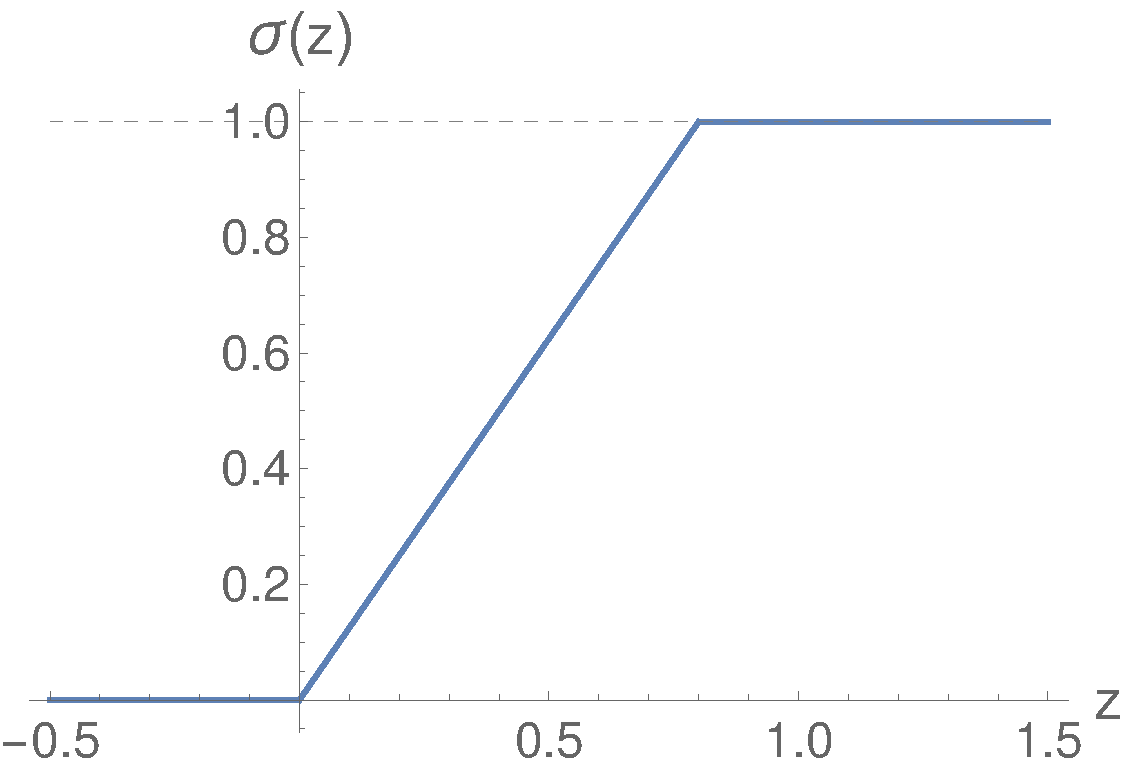
\includegraphics[width=6cm]{actfunc1}}
  \caption{The activation function for $z_{min}=0$, $z_{max}=0.8$.}
\end{figure}


We do not know exactly the way the neurons are adapted to their environment. Thus here we will use a simple model: \textbf{each neuron tries to reach the proportional regime by adjusting their weights}. We will prove that in this way we can in fact create a system that is sensitive to some ``features'' of the input.

We will call a neuron that is in the proportional state (in its operational regime) \emph{fit}, a neuron that is in the $y=0$ regime \emph{negatively stressed}, in the $y=1$ regime \emph{positively stressed}. The above strategy means that a stressed neuron tries to reach its fit state. More precisely we will require that the output is in a narrow vicinity of zero $y\in[\ep, dy]$ where $\ep\ll dy\ll 1$. This interval we be called the strict operating regime, while the fit interval also called weak operating regime.

A natural strategy for the networ could be to set to near zero all of the weights, this automatically forces the output to be small positive value. To avoid it we will require that
\begin{equation}
  \frac1K\sum_{k=1}^K w_k^2 = 1.
\end{equation}

The practical meaning of the above strategy is the folowing:
\begin{itemize}
\item if $y$ lies in the strict operating regime, then we say that the neuron \emph{fully/strictly identifies} its input
\item if $y$ remains in the weak operating regime, then we say that the neuron \emph{weaky identifies} its input
\item if the neuron is stressed, then the neuron misidentifies, or \emph{vetoes} the input. 
\end{itemize}

What is the probability that the neuron identifies its input \emph{by chance}? Let us assume that we have $K$ input neurons, and choose $z_{min}=0$. Let us first use the very simple assumption that all the weights are Gaussian distributed around zero; since they are normalized, each weight has a Gaussian distribution with $0.22\sqrt{K}$ width (if $K$ is large enough). Assuming that the axons are all have the same value $x$, then $z$ has a distribution of $x\sqrt{K}$. The condition that the neuron identifies its input is that $0<z<z_{max}$. This is
\begin{equation}
  \mathop{\mathrm{erf}}(\frac {z_{max}}{x\sqrt{K}})\approx \frac{2z_{max}}{x\sqrt{K\pi}}.
\end{equation}
If $K=20,\,x=0.5$ and $z_{max}=0.1$, this is about $5\%$, but for $x=0.1$ it is just $25\%$. If $x=0.01$ then the probability that a random input is identified is $99.84\%$. That can be interpreted that if the identification of the input occured before (i.e. the earlier axons have small values), than all further layers are unnecessary.

What is said so far, applies for a single neuron. If we have $N$ independent neurons, the probability that \emph{all} identify the input, is $P_1^N$. If we pose a condition that we need at most $P$ probability for misidentification, then
\begin{equation}
  N=\frac{\log P}{\log P_1}.
\end{equation}
Using the above examples, if we want $P=10^{-20}$, and have $K=20,\,x=0.5$ and $z_{max}=0.1$, then we need $N\ge16$ is already enough. For $x=0.1$ we need $N\ge34$ which is still not a very restrictive number. For $x=0.01$, however, we would need $N\approx 30000$ independent neurons, which is already impossible.

\subsubsection{Backpropagation learning}

Let us have a training set $X$ containing the subset we want to learn $X_1\subset X$, and the rest $X_2 = X\setminus X$. We want to develop a network that maps all $x\in X_1$ to a D-dimensional sphere around zero. We may also want that we map $X_2$ to a shell with radius $R$. The network therefore is a function
\begin{equation}
  y_i = N_i(w,x),\qquad i=1,\dots,D,\qquad \frac1K\sum_{k=1}^K w_{k\ell}^2 = 1,\;\forall \ell
\end{equation}
where $\ell$ are the layer indices, $w$ are the weights and $x$ are the inputs.

We can create an expected output: if $x\in X_1$, then $\sum_i y_i^2=0$, if $x\in X_2$ then $\sum_i y_i^2=R^2$. This can summarized into a loss function
\begin{equation}
  L(r) = \frac14 (y^2 - r^2)^2,\qquad y^2 = \sum_i y_i^2.
\end{equation}
Its derivative with respect to $y_i$ reads
\begin{equation}
   \frac{\d L}{\d y_i} = y_i (y^2 - r^2).
\end{equation}
This may be the starting point of backpropagation. The length of this gradient is $y(y^2-r^2)$.

Eventually we may want to add a stochastic component orthogonal to the gradient. If we have a random vector $\xi_i$, and require that it modifies the orthogonal component of a vector $v$, we should have
\begin{equation}
  v'_i = v_i\left(1- \frac{v\xi}{v^2}\right) + \xi_i,
\end{equation}
since then $v'v=v^2$ and $v'v_\perp = \xi v_\perp$.


\subsubsection{Neural learning}

After we have convinced ourselves that neural level learning to reach a smallest possible value is useful strategy, we should provide a mechanism that achieves this goal. Assume that we have inputs $x_k$ and $z=\sum w_kx_k$ (c.f. \eqref{eq:z}). We should compute the derivative of the axon with respect to the weight, but maintaining the constraint that the norm is one.

The direct method is to project the derivative to the orthogonal plane of the constraint. The derivative of the constraint reads
\begin{equation}
  \frac{\d C}{\d w_k} = w_k,
\end{equation}
the orthogonal projector is
\begin{equation}
  \Pi_{k\ell}= \delta_{k\ell}-\frac{w_kw_\ell}K,
\end{equation}
where we used that $\sum_kw_k^2=K$. The derivative of the output reads
\begin{equation}
  \frac{\d y}{\d w_k} = \sigma'(z) x_k,
\end{equation}
so the orthogonal projector is
\begin{equation}
  \Pi_{k\ell}\d_\ell y= \sigma'(z)(x_k - \frac1K w_k z),
\end{equation}
where we used that $z=\sum_kw_kx_k$. But it is also a possibility that we apply a projector at the end by normalizing the weights.

For learning we may use then
\begin{equation}
  \delta w_k = -\alpha \sigma'(z) x_k.
\end{equation}
A technical problem is that $\sigma'(z)=0$ for $z<z_{min}$ and for $z>z_{max}$, while it is $1/\Delta z$ in between. So the steepest descent method does not work correctly. The simplest workaround is that we use an absolute value or a quadratic function instead of $\sigma$. In the second case we obtain
\begin{equation}
  \delta w_k = -\alpha z x_k.
\end{equation}

We may want to make the minimization somewhat stochastic. This can be reached in several ways. We may simply multiply the above change by a random number in the form
\begin{equation}
  \delta w_k = -\alpha(1+\xi_k) \sgn(z)(x_k - \frac1K w_k z),\qquad \exv{\xi_k}=0,\quad \exv{\xi_k\xi_\ell}=W^2\delta_{k\ell}.
\end{equation}
For $W=0$ we get back the earlier result, for large $W$ the update is purely stochastic.

Another possibility is the following. We may define a local energy, and change the weights to minimize it. The point is that it is that the energy can be chosen in any ways provided its minimum coincides the zero gradient result. So we may choose for example
\begin{equation}
  E = \frac12 (w\cdot x)^2 + \lambda (w^2-K)^2.
\end{equation}
The first term tries to minimize $z=w\cdot x$ while the second term forces $w^2=w\cdot w=K$. If $\lambda\gg1$ then the $w^2=K$ constraint is very stiff, practically constraining the minimization to the surface of the $K$-dimensional sphere with radius $\sqrt{K}$.

The energy approach has advantages as opposed to the deterministic equations. First of all we can easily include other requirements. For example, we can choose
\begin{equation}
  E = \frac12 (w\cdot x)^2 + \lambda (w^2-K)^2 + \eta\left[\sum_k x_k (w_k^2-1)\right]^2.
\end{equation}
The second term does not give constraints for the weights, where the input is zero. For example, if only the first $L$ inputs are 1, the rest is 0, then the above energy turns into
\begin{equation}
  E_L = \frac12 (w\cdot x)^2 + \lambda (w^2-K)^2 + \eta\left[\sum_{k=1}^L w_k^2-L\right]^2.
\end{equation}
A possible scenario is that we choose a small $\lambda$ and a large $\eta$. This strognly requires that the weights with large input are not zero (they are near a $L$-dimensional sphere), while weakly require that the weights with zero input are also not zero.

Another possible choice that performs this task is
\begin{equation}
  E = \frac12 (w\cdot x)^2 + \eta\left[\sum_k (x_k+\ep) (w_k^2-1)\right]^2.
\end{equation}

If we want to use steepest descent method to minimize this energy we should go into the direction of the (negative) gradient of the energy. Allowing some stochasticity we may write
\begin{equation}
  \delta w_k = -\alpha \left(\xi_k+ x_k (w\cdot x) + 4 \eta w_k(x_k+\ep) \left[\sum_k (x_k+\ep) (w_k^2-1)\right]\right),
\end{equation}
where $\alpha$ is the learning rate, $\exv{\xi_k}=0$ and $\exv{\xi_k\xi_\ell}=W^2\delta_{k\ell}$ is a noise term.

Alternatively, we may use Monte Carlo technique for update. Single out one weight $w_k$, where the corresponding energy is $E$. We choose a new weight $w_k'$, then the corresponding energy we denote by $E'$. We accept the new weights with probability
\begin{equation}
  P_{acc} = \min\left(1, e^{-\beta(E'-E)}\right).
\end{equation}
If $\beta=0$, then we always accept the new weight (infinite temperature), if $\beta=\infty$, then we accept it only if $E'<E$ (zero temperature). With this method we can ensure that the distribution of the weights is
\begin{equation}
  P(w) \sim e^{-\beta E}.
\end{equation}


\subsection{Examples of activation functions}

  
  \begin{eqnarray}
    && \sigma = \frac12\left(\frac {\beta x}{\sqrt{\beta^2x^2+1}}+1\right);\qquad \sigma' = \frac \beta{2\sqrt{1+\beta^2x^2}} = 4\beta(\sigma(1-\sigma))^{3/2}\nn
    && \sigma = \frac12\left(1+\tanh \beta x\right) = \frac1{1+e^{-2\beta x}}; \qquad \sigma' = \frac{2\beta e^{2\beta x}}{(1+e^{2\beta x})^2} = 2\beta\sigma(1-\sigma)\nn
    && \sigma = \left\{
       \begin{array}[c]{rl}
         0,\quad & \mathrm{if}\; x<-\frac\pi{2\beta}\cr
         (1+\sin \beta x)/2,\quad & \mathrm{if}\; -\frac\pi{2\beta}<x<\frac\pi{2\beta}\cr
         1,\quad & \mathrm{if}\; x>\frac\pi{2\beta}.\cr
       \end{array} \right\};\qquad
          \sigma' = \left\{
       \begin{array}[c]{rl}
         0,\quad & \mathrm{if}\; x<-\frac\pi{2\beta}\cr
         \beta /2\cos \beta x,\quad & \mathrm{if}\; -\frac\pi{2\beta}<x<\frac\pi{2\beta}\cr
         0,\quad & \mathrm{if}\; x>\frac\pi{2\beta}.\cr
       \end{array}
       \right\} = \beta\sqrt{\sigma(1-\sigma)},\nn
    && \sigma = \left\{
       \begin{array}[c]{rl}
         0,\quad & \mathrm{if}\; x<-\frac1\beta\cr
         (1+\beta x)/2,\quad & \mathrm{if}\; -\frac1\beta<x<\frac1\beta\cr
         1,\quad & \mathrm{if}\; x>\frac1\beta.\cr
       \end{array} \right\};\qquad
          \sigma' = \left\{
       \begin{array}[c]{rl}
         0,\quad & \mathrm{if}\; x<-\frac1\beta\cr
         \beta /2,\quad & \mathrm{if}\; -\frac1\beta<x<\frac1\beta\cr
         0,\quad & \mathrm{if}\; x>\frac1\beta.\cr
       \end{array}
       \right\} = \frac\beta2\Theta[\sigma(1-\sigma)],\nn
  \end{eqnarray}
  The derivative of all of these functions is $\beta/2$ at the origin. The plot of these functions is shown in Fig.~\ref{fig:actfunc} for $\beta=1$.
  \begin{figure}[htbp]
    \label{fig:actfunc}
    \centerline{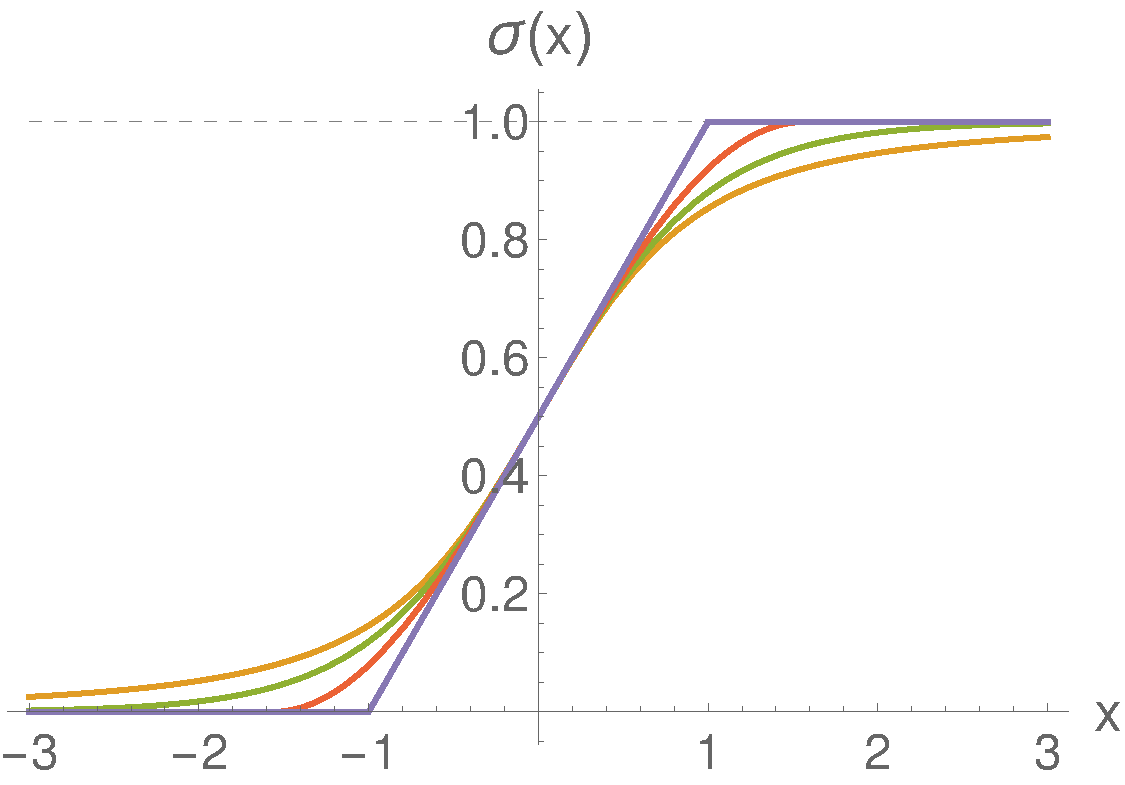
\includegraphics[width=6cm]{actfunc}}
    \caption{The activation functions for $\beta=1$.}
  \end{figure}
  As we see from the derivatives, all of the above activation functions are member of a common family with $\sigma'=\beta/2(4\sigma(1-\sigma))^\alpha$ for different $\alpha$.


\end{document}
